% TeX root=../main.tex

A inscrição (\autoref{fig:bohça}) é conhecida desde 1901, tendo sido encontrada
em uma colina do vilarejo de Bohça (Bozca ou Bahçeköy),
provavelmente no contexto original e está atualmente locada no Kayseri
Arkeoloji Müzesi (no.\ 6).
O governante Kurtis filho de Ashwisis talvez possa ser identificado com o
mesmo governante mencionado por Sargão II por Kurti de Atunna entre 718--713
\textsc{aec}, e o estilo da inscrição corresponde ao esperado para este
período.
A associação, no entanto, depende da localização de Atunna.
Bohça está no meio da região conhecida das fontes
neo-assírias pelo nome de Tabal que, na idade do ferro, era composta por
diversas pequenas cidades-estado.

\begin{center}
	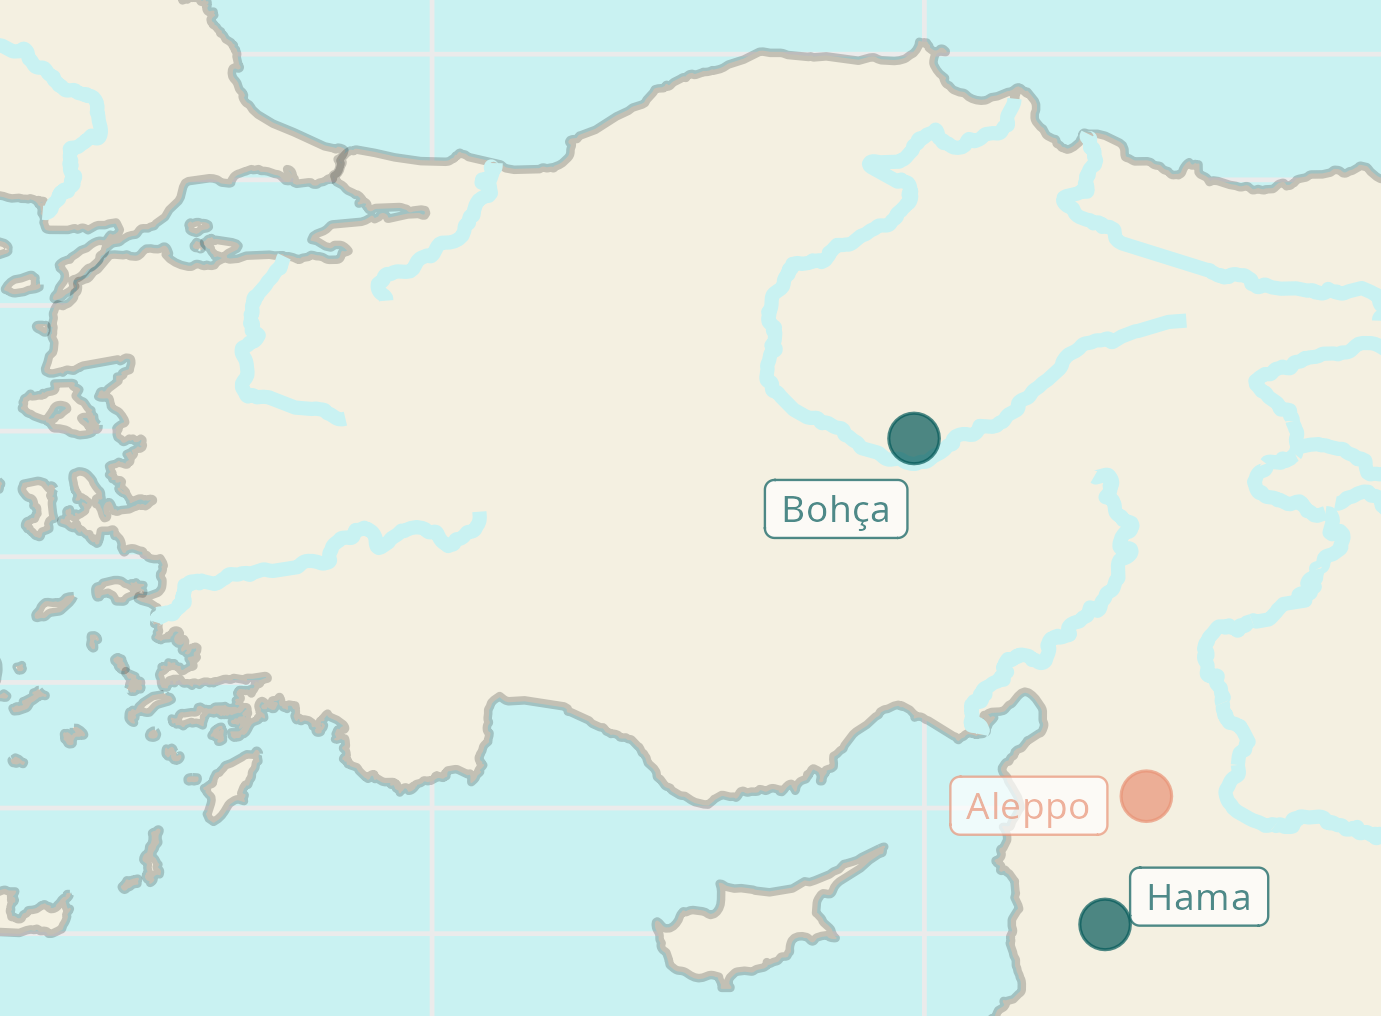
\includegraphics[width=0.65\textwidth]{../../../Mídia/Map03.png}
\end{center}


\begin{figure}[h]
	\centering
	\begin{subfigure}{0.49\textwidth}
		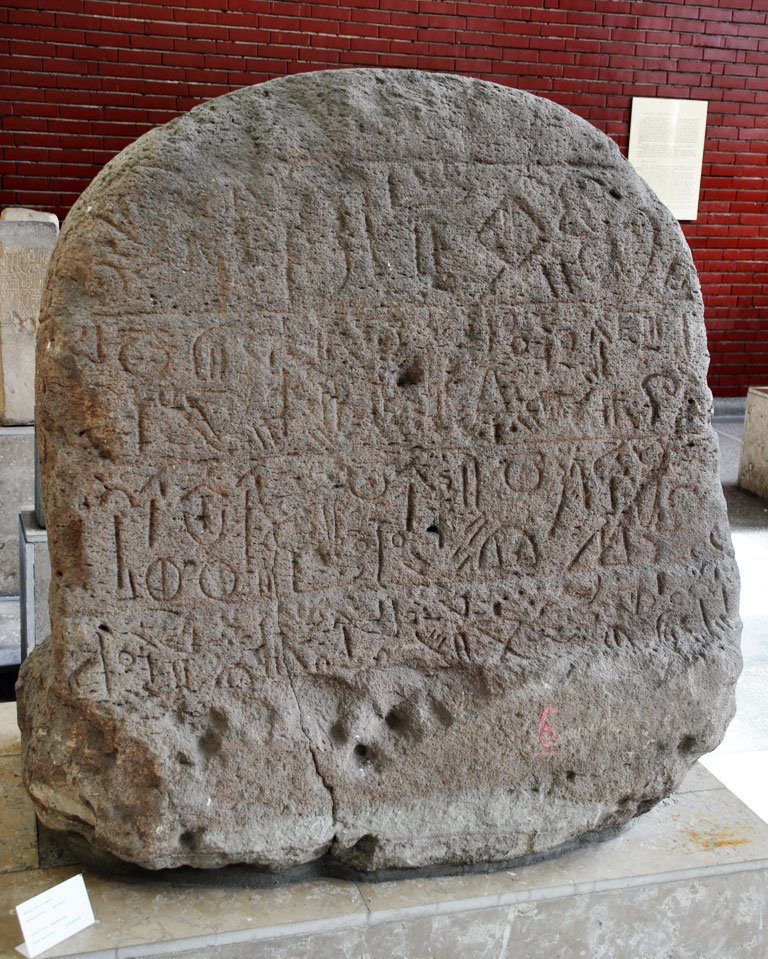
\includegraphics[width=0.9\textwidth]{../../../Mídia/bahce08.jpg}
	\end{subfigure}
	\hfill
	\begin{subfigure}{0.49\textwidth}
		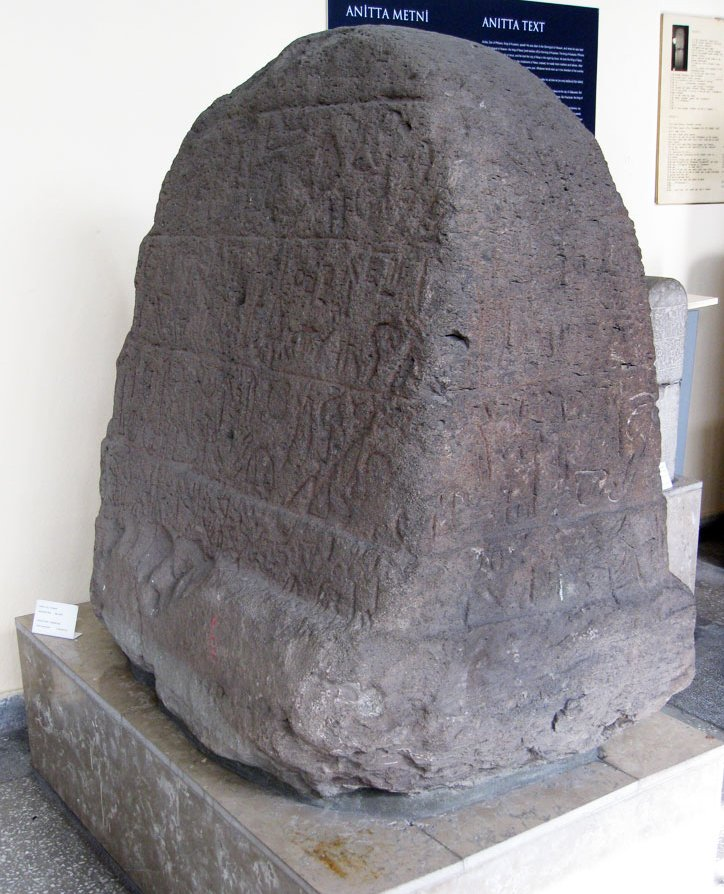
\includegraphics[width=0.9\textwidth]{../../../Mídia/bahce10.jpg}
	\end{subfigure}
	\caption[BOHÇA]{Inscrição BOHÇA. Dimensões da inscrição:
		1.26\times0.63m.
		Imagens de Cüneyt Süer, 2011,
		disponíveis em
		\href{https://www.hittitemonuments.com/bahcekoy/}{Hittite Monuments}.
		Edição e traçado em~\citeabbrev*{CHLI11}, pp.\ 478ff.\ e \emph{plate}
		265.
	}\label{fig:bohça}
\end{figure}

\clearpage

\begin{center}
	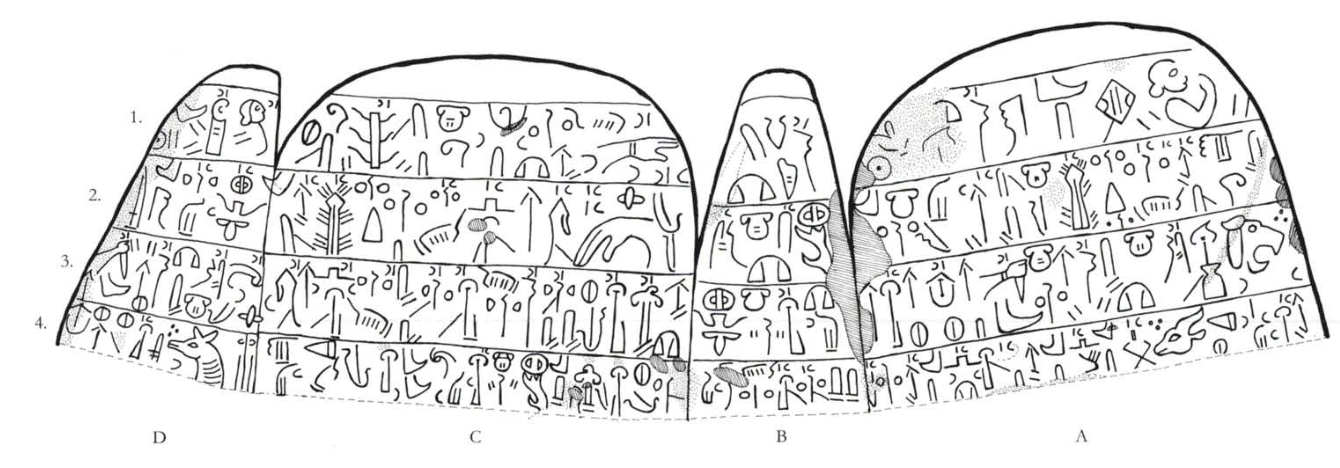
\includegraphics[width=\textheight,angle=90]{../../../Mídia/bohça.png}
\end{center}


\setcounter{parcount}{0}
\begin{parnumbersa}[]

	\raggedright%
	\itshape%

	\logo{EGO}-wa/i-mi \spac{}ka-tú-wa/i-sa \logo{“IUSTITIA”}-ni-i-sa
	\logo{DEUS}-ni-ti-i \logo{(LITUUS)}á-za-mi-i-sa
	kar-ka-mi-si-za-sa\logo{(URBS)} \lmasc{}\logo{REGIO}-ni \logo{DOMINUS}-sa
	\spac{}su-hi-si \lmasc{}\logo{REGIO}-ni \logo{DOMINUS}-ia-i-sa
	\lmasc{}\logo{FILIUS.}NI-za-sa \spac{}á-sa-tú-wa/i-lá/í-ma-za-si \logo{REGIO}-ni \logo{DOMINUS}-i-sa \lmasc{}\logo{FILIUS.NEPOS}-si-i-sa

	a-wa/i za-a-sa \logo{URBS+}MI-ni-i-sa mi-sá-*a \lmasc{}tá-da-li-sa
	\logo{AVUS}-ha-da-li-sa \lbreak{} \spac{}\logo{*447}-nu-wa/i-ia-si sa-tá-*a

	wa/i-sa-*a \logo{VACUUS}-ti-i-sa \lmasc{}\logo{ARHA} \logo{(“LONGUS”)}ia\logo{+} ra/i-ia-ta

	wa/i-na-*a \spac{}\logo{MAGNUS+}ra/i-\logo{TONITRUS}-tá-sa-za \lmasc{}\logo{FILIUS.NEPOS}-sa-za \logo{CUM}-ní \lmasc{}\logo{(LOCUS)}pi-ta-ha-li-ia-ha

	wa/i-ma-zá-*a mi-i-na-*a \lmasc{}sá-pa-la/i-li-na \lmasc{}\logo{URBS+}MI-ni i-pa-ni-si-ná\logo{(URBS)} \lmasc{}á-ma-ha-wa/i \lmasc{}sá-pa-lá/í-li-ia \logo{TERRA.PONERE}-ru-da mu-zi-ki-ia\logo{(URBS)} \lmasc{}$[$\logo{\ldots{}}$]$ \lbreak{}

	wa/i-ma-na-a* \lmasc{}\logo{AEDIFICARE}-\logo{MI}-ha

	a-wa/i \lmasc{}\logo{REL}-a-ti-i \lmasc{}\logo{(ANNUS)}u-si-i
	ka-wa/i-za-na\logo{(URBS)} \lmasc{}\logo{(CURRUS)}wa/i\logo{+}ra/i-za-ni-ná
	\lmasc{}\logo{PES\textsubscript{2}}-za-ha

	pa-tá-za-pa-wa/i-ta-*a \logo{(TERRA+LA+LA)}wa/i-li-li-da-za mi-i-zi-*a
	\lmasc{}tá-ti-i-zi \logo{AVUS}-ha-ti-zi-ha
	\lmasc{}\logo{*348}{(-)}lu/a/i\textsuperscript{?}-da-li-zi-ha
	\lmasc{}\logo{NEG\textsubscript{2}}-a \logo{(PES\textsubscript{2})}hwi/a-hwi/a-sà-tá-si

	mu-pa-wa/i-*a mi-i-sa-*a \logo{(DOMINUS)}na-ní-i-sa \lbreak{} \logo{CAELUM} \logo{(DEUS)}\logo{TONITRUS}-sa \logo{(DEUS)}kar-hu-ha-sá \logo{(DEUS)}ku\logo{+AVIS}-pa-pa-sa-ha mi-ia-ti-*a \logo{“IUSTITIA”}-wa/i-na-ti \logo{(LITUUS)}á-za-tá

	wa/i-ma-tá-*a \logo{(“LIGNUM”)}hu-hú\logo{+}ra/i-pa-li \lmasc{}\logo{(SOLIUM)}á-sa-tá

	wa/i-ma-da-*a \lmasc{}\logo{PRAE}-na \logo{(PES\textsubscript2)}hwi/a-ia-ta

	a-wa/i pa-ia-*a \lmasc{}\logo{REGIO}-ni-ia \logo{(“VACUUS”)}ta-na-tá-ha

	wa/i-ta-*a \logo{(SCALPRUM.CAPERE2)}u-pa-ní-zi a-tá \lmasc{}\logo{(“CAPERE2”)}\lbreak{}u-pa-ha

	a-wa/i pi-i-na-*a \lmasc{}\logo{REGIO}-ni-ia-ti \logo{(FULGUR)}pi-ha-mi-sa \logo{SUPER+}ra/i-a \lmasc{}\logo{PES}-wa/i-i-ha

	\lmasc{}za-zi-ha-wa/i-mi-i \logo{(DOMUS.SUPER)}ha\logo{+}ra/i-sà-tá-ni-zi pa-ti-i-*a \logo{(“ANNUS”)}u-si \lmasc{}\logo{AEDIFICARE}-\logo{MI}-ha

	wa/i-mi-ta-*a mi-i-na-*a \logo{(DOMINUS)}na-<<i>>-ni-i-na \logo{(DEUS)}kar-hu-ha-si-na \logo{(DEUS)}ku\logo{+AVIS}-pa-si-ha \logo{CRUS2}\logo{.CRUS}{(-)}ní-ia-sa-ha-na \lmasc{}\logo{LITUUS+}na-ha

	wa/i-ma-tá-*a \lmasc{}za\lbreak{}-ti-i \lmasc{}\logo{(“PODIUM”)}hu-ma-ti \lmasc{}\logo{(SOLIUM)}i-sà-nú-wa/i-ha

	\logo{(“*350”)}á-sa-ha\logo{+}ra/i-mi-sà-pa-wa/i-ma-za \lmasc{}za-a \logo{DEUS}-ní-za
	\lmasc{}\logo{CUM}-ni \logo{ANNUS}-sa-li-za-sa
	\lmasc{}\logo{(“PANIS”)}tú\logo{+}ra/i-pi-sa
	\logo{(DEUS)}\logo{CERVUS\textsubscript{3}+}ra/i-hu-ha-ia 1
	\logo{BOS}\logo{(ANIMA)}-sa \logo{OVIS}-sa-ha
	\logo{(DEUS)}ku\logo{+AVIS}-pa-pa 1 \logo{BOS}\logo{(ANIMA)}-sa 1
	\logo{OVIS}\logo{(ANIMA)}-wa/i-sa-ha
	\logo{(DEUS)}sa\textsubscript{5}\logo{+}ra/i-ku \logo{OVIS}-wa/i-sa \logo{(“*478”)}ku-tú-pi-li-sa-ha 1 \logo{OVIS}\logo{(ANIMA)}-wa/i-sa \lmasc{}\logo{VIR}-ti-ia-da-za \logo{DEUS}-ní-za \lbreak{} $[$1 \logo{OVIS}\logo{(ANIMA)}-wa/i$]$-sa $[$\logo{FEMINA}-ti$]$-ia-$[$ta$]$-za $[$\logo{DEUS}-ni-za$]$

	$[$\logo{\ldots{}}$]$-sa z$[$a-ti$]$-ia-za $[$\logo{DEUS}-n$]$i\textsuperscript{?}-za \logo{MALUS}-la/i-ti-i-*a \lbreak{} \logo{VERSUS}-ia-ni \lmasc{}\logo{PES}-wa/i-ti

	\lmasc{}\logo{NEG\textsubscript{2}}-pa-wa/i-sa \lmasc{}za-ti-ia-za \logo{(DOMUS.SUPER)}ha\logo{+}ra/i-sà-tá-na-za \logo{MALUS}-la/i-ti-i-*a \lmasc{}\logo{VERSUS}-ia-ni $[$\logo{PES}$]$-wa/i-ti

	$[$\lmasc{}$]$\logo{NEG\textsubscript{2}}-$[$pa$]$-wa/i-da
	\logo{CRUS2.CRUS}$[${(-)}ni\textsuperscript{?}$]$-ia-za-i \logo{REL}-a-ti \logo{PRAE}-na

	$[$wa/i$]$-da-*a $[$\logo{SCRIBA+RA/I}$]$\logo{CAPERE}/da-\textsc{⌈}i\textsc{⌉} \textsc{⌈}\lmasc{}\textsc{⌉}\logo{REL}-i-sa

	\lmasc{}za-a-zi-pa-wa/i-tá
	$[$\logo{(SCALPRUM)}$]$ku-ta-sa\textsubscript{5}\logo{+}ra/i-zi-i
	\logo{LOCUS}-la/i-za-\textsc{⌈}*a\textsc{⌉} [\textsuperscript{?}]\lbreak{}-i-t[i]

	\lmasc{}\logo{NEG\textsubscript{2}}-pa-wa/i-tá \lmasc{}za-a-ti-ia-za
	\lmasc{}\logo{(“SCALPRUM”)}ku-ta-sa\textsubscript{5}\logo{+}ra/i-za \lmasc{}á-ma-za \lmasc{}á-lá/í-ma-za \lmasc{}\logo{ARHA} \lmasc{}\logo{“MALLEUS”}-lu/a/i-i

	pa-ti-pa-wa/i-tá-*a \logo{CAELUM} \logo{(DEUS)}\logo{TONITRUS}-sa \logo{(DEUS)}kar-hu-ha-sá \logo{(DEUS)}ku\logo{+AVIS}-pa-pa-sá-ha \logo{(MONS)}a\logo{+}ra/i-pu-tá-wa/i-ni-sá-ha \logo{(DEUS)}\logo{TONITRUS}-sa \logo{(“FLUMEN+MINUS”)}sà-ku\logo{+}ra/i-wa/i-ni-i-zi-ha \logo{(FLUMEN.REGIO)}ha\lbreak{}-pa-da-si \logo{DEUS}-ní-zi \lmasc{}\logo{LIS}-lu/a/i-sa-tú

	wa/i-tú-*a \lmasc{}\logo{VIR}-ti-ia-ti-ia-za-ha \lmasc{}\logo{(“CULTER”)}pa\logo{+}ra/i-tú-ní-tú-u

	\logo{FEMINA}-ti-ia-ti-ia-za-ha-wa/i-tú-u \lmasc{}\logo{(“CULTER”)}pa\logo{+}ra/i-tú-ni-i-tú

	wa/i-tú-*a \lmasc{}\logo{VIR}-ti-ia-ti-i-na \lmasc{}\logo{(*462)}mu-wa/i-i-da-na \logo{NEG3}-sa \lmasc{}\logo{CAPERE}-ti-i

	\logo{FEMINA}-ti-i$[$a$]$-ti-pa-wa/i-tú
	\logo{(FEMINA.*462)}\lbreak{}{4}\textsuperscript{?}-da \lmasc{}ni-i \lmasc{}\logo{CAPERE}-ti-i

	\lmasc{}za-pa-wa/i-tá \lmasc{}\logo{URBS+}MI-ni-i-na mu-*a
	\lmasc{}\logo{REL+}ra/i-i \spac{}\logo{MAGNUS+}ra/i-\logo{TONITRUS}-ta-sa-za
	\lmasc{}\logo{FILIUS.NEPOS}-sa-za \lmasc{}\logo{(“*314”)}ha-sá-ti-i \logo{ARHA} \lmasc{}\logo{CAPERE}-ha

	\lmasc{}\logo{NEG\textsubscript{2}}-wa/i-na \lmasc{}\logo{REL+}ra/i-i \logo{(LOCUS)}pi-ta-ha-li-ia-ha

	a-wa/i \lmasc{}za-a-zi \lmasc{}\logo{DEUS}-ní-i-zi \lmasc{}\logo{AUDIRE+MI}-ta\logo{+}ra/i-ru

	\logo{“LIGNUM”}-sa-pa\lbreak{}-wa/i-mu-tá-a \lmasc{}\logo{REL}-a-za za-a-ti-ia-za \lmasc{}\logo{(DOMUS.SUPER)}ha\logo{+}ra/i-sà-tá-na-za \logo{POST}-ni \lmasc{}\logo{PES}-wa/i-da

	a-wa/i \lmasc{}za-a-zi \logo{“PORTA”}-lu/a/i-ni-si-i-zi
	\logo{(DOMUS.SUPER)}ha\logo{+}ra/i-sà-tá-ní-zi \spac{}á-na-ia mi-i-*a
	\lmasc{}\logo{BONUS}-sa-mi-i \logo{FEMINA}-ti-i
	\lmasc{}\logo{(BONUS)}wa/i-sa\textsubscript{5}\logo{+}ra/i-ti-i pa-ti-i-*a \lmasc{}\logo{(ANNUS)}u-si-i \logo{AEDIFICARE}-\logo{MI}-h$[$a$]$


\end{parnumbersa}

\clearpage

\setcounter{parcount}{0}
\begin{parnumbersa}[]

	\raggedright%
	\itshape%

	amu=wa=mi Katuwas, tarawanis, masanidi azamis, Karkamisizas
	\logo{REGIO}-ni-\logo{DOMINUS}-s,
	Suhisi \logo{REGIO}-ni-\logo{DOMINUS}-yais nimuwizas,
	Asatuwalamanzasi \logo{REGIO}-ni-\logo{DOMINUS}-is hamsis.

	a=wa zas \logo{URBS+}MI-nis tadallis huhadallis Ninuwis asta.

	a=wa=as tanatis arha yariyata.

	a=wa=an Uratarhuntasanza hamsanza \logo{CUM}-ni pitahaliyaha.

	a=wa=manza amin sapalalin \logo{URBS+}MI-nin Ipanisin, ama=ha=wa sapalaliya
	\logo{TERRA.PONERE}-ruda Muzikiya \ldots{}

	a=wa=mw=an tamaha.

	a=wa kwati usi Kawazan warazanin wazaha,


	apatanza=pa=wa=ta walilidanza aminzi tatinzi huhatinzi=ha \logo{*348}-dalinzi=ha na hwihwisantasi

	amu=pa=wa nanis tipasis Tarhuntas, Karhuhas, Kubabas=ha amiyati tarwanadi
	azanta.

	a=wa=mw=a\emph{t}a huhurpali asanta,

	a=wa=mw=ada paran hwiyanta.

	a=wa apaya \logo{REGIO}-niya tanataha.


	a=wa=ta upaninzi anta upaha.

	a=wa apin \logo{REGIO}-niyadi pihamis sara awiha.

	zanzi=ha=wa=mi haristaninzi apati usi tamaha.

	a=wa=mi=ta amin nanin Karhuhasin Kubabasin=ha niyashan \logo{LITUUS}+naha.

	a=wa=mw=ata zati humati isanuwaha.

	asharimis=pa=wa=manza za masani{(ya)}nza \logo{CUM}-ni usalizas turpis:
	Karhuhaya 1 wawis hawas=ha;
	Kubaba 1 wawis hawas=ha;
	Sarku hawas kutupilis=ha;
	1 hawas zidiyadanza masani{(ya)}nza; $[$1 hawa$]$s $[$wanati$]$ya$[$ta$]$nza
	masani{(ya)}nza.


	$[$kwis$]$-s za$[$ti$]$yanza $[$masani$]${(ya)}nza atuwalidi
	tawiyan awati,

	napa=wa=as zatiyanza haristananza atuwalidi tiwiyan $[$a$]$wati,

	na$[$pa$]$=wa=ada $[$ni$]$yazai kwati paran,

	a=$[$wa$]$=ada \logo{SCRIBA+}ra-\logo{CAPARE}dai kwis,

	zanzi=pa=wa=ta kutasarinzi arlanza {?}-iti

	napa=wa=ta zatiyanza kutasari{(ya)}nza amanza alamanza arha walai,

	apati=pa=wa=ta tipasis Tarhuntas, Karhuhas, Kubabas=ha, arputawanis=ha
	Tarhuntas, Sakurawaninzi=ha hapadasi masaninzi \logo{LIS}-lu/a/i-santu.

	a=wa=tu zidiyadiya=za partunintu,

	wanatiyatiya=za=ha=wa=tu partunintu.

	a=wa=tu zidiyadin muwidan nis lanti,

	wanatiyatin=pa=wa=tu muwidan ni lanti.

	zan=pa=wa=ta \logo{URBS+}MI-nin amu kwari Uratarhuntasanza hamsanza hasadi arha laha

	na=wa=an kwari pitahaliyaha,

	a=wa zanzi masaninzi tumantintaru.

	taruwis=wa=mu=ta kwanza zatiyanza haristananza apan awada,

	a=wa zanzi \logo{PORTA}-lanisinzi haristanninzi Anaya ami wasami wanati wasaradi
	apati usi tamaha.


\end{parnumbersa}

[1] Eu sou Katuwa, justo, amado pelos deuses, senhor regional de Karkamis, filho
de Suhis, o senhor regional, neto de Asatuwalamaza, o senhor regional.
	[2] Esta cidade do meu pai e avô era\slash{}tornou-se (de?) Ninuwi,
[3] E ela esticou-se em vão {???.}
[4] E com os netos de Uratarhunta eu PITAHALIYA-ei,
[5] E para eles minha cidade SAPALALI Ipanis e minhas SAPALALI-s {???} Muzikis {???}.
[6] Eu mesmo a construí,
[7] no ano em que eu movi a campanha pela cidade de Kawaza,
[8] para aqueles territórios meus pais, avós, bisavós não marcharam.

	[9] Mas a mim o senhor celeste Tarhunta, Karhuha e Kubaba pela minha justiça
amavam,
[10] eles me sentaram no HUHURPALA,
[11] eles correram na minha frente
	[12] e eu destruí aquelas regiões.

[13] Eu trouxe prêmios para dentro,
[14] eu voltei glorioso daquelas regiões,
[15] e estes andares superiores eu construí naquele ano.

	[16] E eu vi pessoalmente a procissão do meu senhor Karhuha e Kubaba,
[17] e eu mesmo os sentei neste altar.

	[18] O sacrifício de sangue para estes (seja):
para os deuses em conjunto, o pão anual;
para Karhuha, 1 touro e uma ovelha;
(para) Kubaba, 1 touro e uma ovelha;
(para) Sarku, uma ovelha e um KUTUPILI\@;
1 ovelha para os deuses masculinos;
1 ovelha para as deusas femininas.

\ldots{}

[19] Aquele que se aproximar destes deuses com maldade,
[20] ou que se aproximar desses andares superiores com maldade,
[21] ou se eles seguirem {?}para baixo / {?}transferirem a alguém,
[22] que {???}
	[23] e que {???} estas estelas do seus lugares,
[24] ou apague meu nome dessas estelas,
[25] contra ele o celeste Tarhuta, Karhuha, Kubaba, Tarhunta do Monte Arputa e
os deuses da terra fluvial do rio Sakura litiguem!

[26] Que dele arranquem a masculinidade,
[27] que dela arranquem a feminilidade,
[28] que dele eles não tomem a semente masculina,
[29] que dela eles não tomem a semente feminina.

	[30] Se eu mesmo tomei esta cidade dos netos de Uratarhunta à força,
[31] e se ela eu não PITAHALIYA-ei,
[32] sejam estes deuses testemunhas.

	[33] Porque a madeira para estes andares superiores chegou depois para mim,
[34] estes andares superiores dos portais à Ana, minha boa mulher, com bondade
construí naquele ano.



